\documentclass[a4paper,12pt]{article} % тип документа
\usepackage[margin=1in]{geometry} % Поля

%  Русский язык
\usepackage[warn]{mathtext}
\usepackage[T2A]{fontenc}			% кодировка
\usepackage[utf8]{inputenc}			% кодировка исходного текста
\usepackage[english,russian]{babel}	% локализация и переносы
% Математика
\usepackage{amsmath,amsfonts,amssymb,amsthm,mathtools} 
\usepackage{wasysym}
%%%
\usepackage{graphicx}

\usepackage{tabularx}

\usepackage{gensymb} % знак градуса
\usepackage{enumitem} % изменить список enumerate
\usepackage{placeins} % \FloatBarrier

\renewcommand{\thesection}{\Roman{section}} 
\renewcommand{\thesubsection}{\roman{subsection}}
\renewcommand{\thesubsubsection}{\roman{subsection}.\roman{subsubsection}}


\begin{document}

\newcolumntype{Y}{>{\centering\arraybackslash}X} %new tabularx


%титул

\begin{center}
{\LARGE Московский Физико-Технический Институт}
\\
{\large Физтех-школа электроники, фотоники и молекулярной физики }
\\
\vspace{8cm}
{\LARGE Отчёт по лабораторной работе:}
\\
{\Huge Конвективная диффузия в молекулярно- электронных преобразователях} 
\\
\vspace{5cm}
\raggedright 
\hspace{7cm}{\large Выполнили студенты группы Б04-005}\\
\hspace{7cm}{\large Карташов Констанин}\\
\hspace{7cm}{\large Давыдов Владислав}\\
\hspace{7cm}{\large Корнеев Николай}\\
\hspace{7cm}{\large Голощапов Михаил}

\vspace{\fill}
\center
{\large Долгопрудный 2022}

\end{center}

\newpage


\section{Анотация}

\paragraph{Цель работы:} 
изготовить контакты алюминия с кремнием n- и p-типов, снять вольтамперную характеристику диода Шоттки, построить ее в полулогарифмическом масштабе, рассчитать высоту барьера, построить вольтамперную характеристику омического контакта.
\paragraph{Оборудование:}
\begin{itemize}
\renewcommand{\labelitemi}{$\triangleright$}
\itemsep0em
\item Вакуумная установка,
\item Газоразрядная трубка,
\item Лабораторный блок питания.
\end{itemize}



\medskip\hrule\medskip

\section{Теоретические сведения}
\subsection{Энергетические диаграммы}
В данной работе нам предстоит работать с процесами, истекающими из внутренего энергетического строения металлов и полупроводников. Чтобы понять это строение посмотрим на энергетические диаграммы:
\begin{figure}[h!]
    \centering
    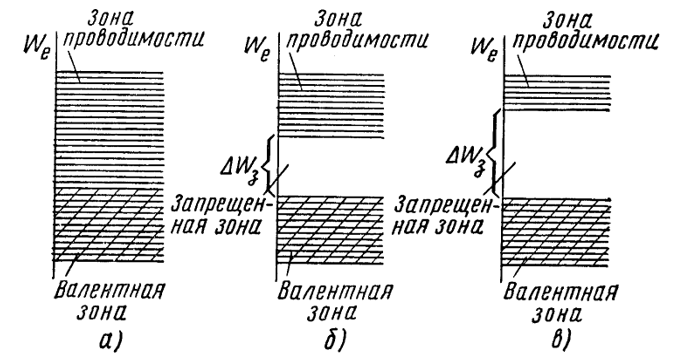
\includegraphics[width=15cm]{energ_1.png}
        \caption{Энергетические диаграммы металла, полупроводника и диэлектрика}
    \label{1}
\end{figure}
\begin{itemize}
    \itemВ металле зона проводимости и валентная зона пересекают друг друга (рис.\ref{1}а), сама диаграмма металла представляет собой потенциальную яму глубиной $\varphi_F$ - энергия Ферми. Уровень Ферми может меняться в зависимости от внешних условий.
    \itemВ полупроводнике вся диаграмма разделена на три зоны: зона проводимости, запрещенная зона и валентная зона. При нулевой температуре все электроны находятся в самой нижней валентной зоне, а уровень Ферми находится посередине запрещенной зоны. С увеличением температуры электроны становятся способны преодолеть запрещенную зону и находиться в зоне проводимости, это конечно заставляет уровень Ферми сближаться к зоне проводимости.\\
Полупроводники возможно легировать примесью, это ожидаемо меняет его энергетическую диаграмму.\\
Если легировать полупроводник примесями с n-проводимостью, то полупроводник получает лишние электроны с энергией соответсвующей верхней части запрещенной зоны, следовательно данные электроны легко могут перейти в зону проводимости и сместить уровень Ферми "вверх".\\
В случае легирования примесью с p-проводимостью акцепторная примесь захватывает электроны из валентной области, таким образом эти электроны остаются там и уровень Ферми смещается "вниз".

\end{itemize}

\subsection{Потенциальный барьер металл-полупроводник}
\begin{figure}[h!]
    \centering
        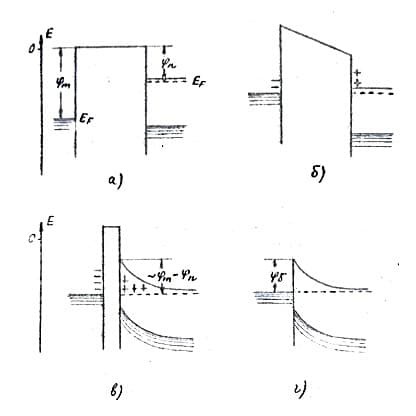
\includegraphics[width=10cm]{energ_2.jpg}
    \caption{Энергетические диаграммы металла и полупроводника}
    \label{2}
\end{figure}
Возьмем металл и полупроводник, так что $\varphi_m>\varphi_n$. Если мы приведем их в контакт (например, соединим проволкой), то электроны из зон проводимости полупроводника начнут переходить в металл пока уровни Ферми не сравняются (\ref{2}б). Это в свою очередь приведет к разности потенциалов между ними: $U=\frac{(\varphi_m-\varphi_n)}{e}$. \\
\indentТеперь сблизим наши образцы - электрической поле между ними будет возрастать и в какой-то момент станет достаточно большим, чтобы воздействовать на внутрее строение полупроводника. Зоны внутри полупроводника начинают искривляться (\ref{2}в), что в свою очередь образует дополнительный потенцал равный $U$. Электроны покидают поверхностные области полупроводника и образуют обедненные слои.\\
\indentОбразовавшийся барьер Шоттки позволяет только электронам с достаточно большой энергией совершать обмен. Ток, создаваемый этими электронами, описывается по формуле термоэлектронной эмиссии:
\begin{equation}
    I_0=SA_0T^2e^{-\frac{\varphi}{kT}}
\end{equation}
Общий ток является суммой двух токов, идущих с противоположных сторон. Поэтому при отсутствии внешнего напряжения общий ток равен нулю. Однако если подать напряжение, то оно в основном затронет обедненный слой, что в свою очередь изменяет высоту барьера. Из-за этого процесса пропускная способность диода Шоттки является односторонней и ток описывается формулой:
\begin{equation}
    I=I_0(e^\frac{eU}{kT}-1)
\end{equation}
\indentВсе это время мы рассматривали случай, когда $\varphi_m>\varphi_n$. Если это не так, то электрическое поле будет направленно в другую сторону, следовательно, искривление происходит в другую сторону. Что в свою очередь образует "обогащенный" слой вместо обедненного с большой проводимостью. Потенциальный барьер в этом случае отсутствует, следовательно при достаточно малых токах контакт можно считать омическим.

\medskip\hrule\medskip

\section{Экспериментальная часть}

ВАХ снимали с готовых образцов (рис. \ref{fig:micro}) (в виду неисправности установки свои диоды сделать не получилось): кремний, легированный фосфором и покрытый с обеих сторон алюминием (Al – nSi–Al) и легированный бором и покрытый с одной стороны алюминием, а с другой – золотом (Al–pSi–Au). На первом образце наблюдался контакт Шоттки, а на втором – омический. 
Построим ВАХ на основе получившихся значений для контакта Шоттки и омического контакта.

    \begin{figure}[h!]
		\centering
		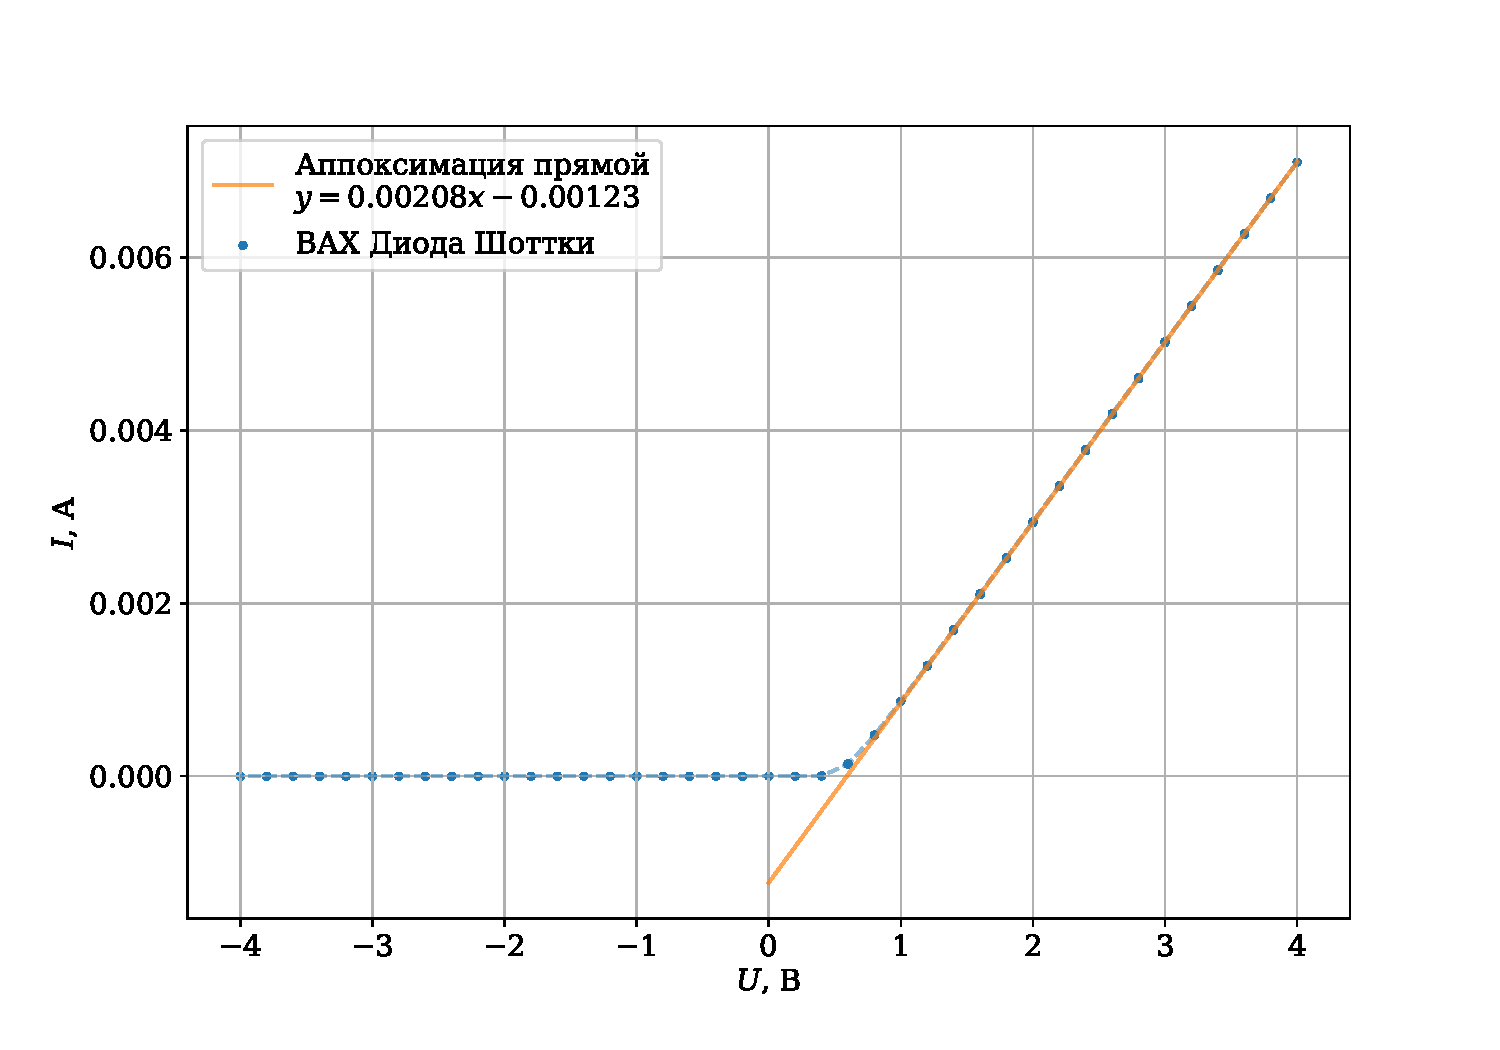
\includegraphics[width=\textwidth]{vac_diode.pdf}
		\caption{ВАХ контакта Шоттки}
		\label{graph1}
	\end{figure}
	
	\begin{figure}[h!]
		\centering
		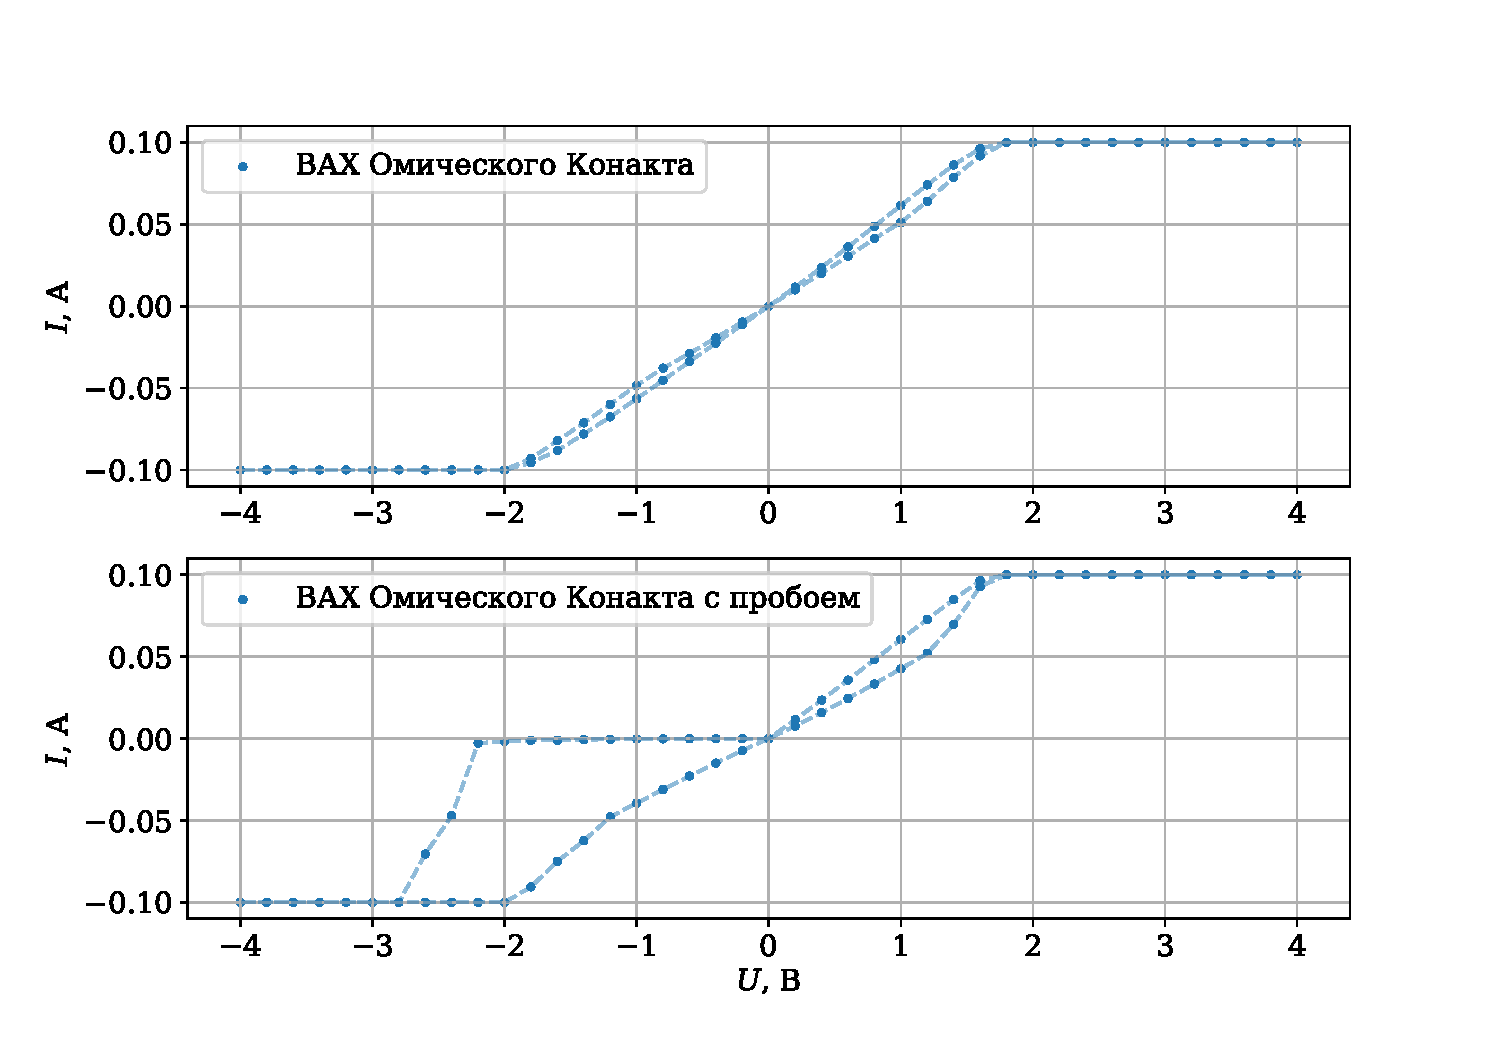
\includegraphics[width=\textwidth]{vac_ohm.pdf}
		\caption{ВАХ омического контакта}
		\label{graph2}
	\end{figure}
	
Построим ВАХ контакта Шоттки в полулогарифмическом масштабе. Прямолинейный участок аппроксимируем выражением:

\begin{equation}
    \ln{I}= \ln{SA_0 T^2} - \frac{\varphi_b}{k_B T} + \frac{e}{\gamma k_B T} U
\end{equation}

	\begin{figure}[h!]
		\centering
		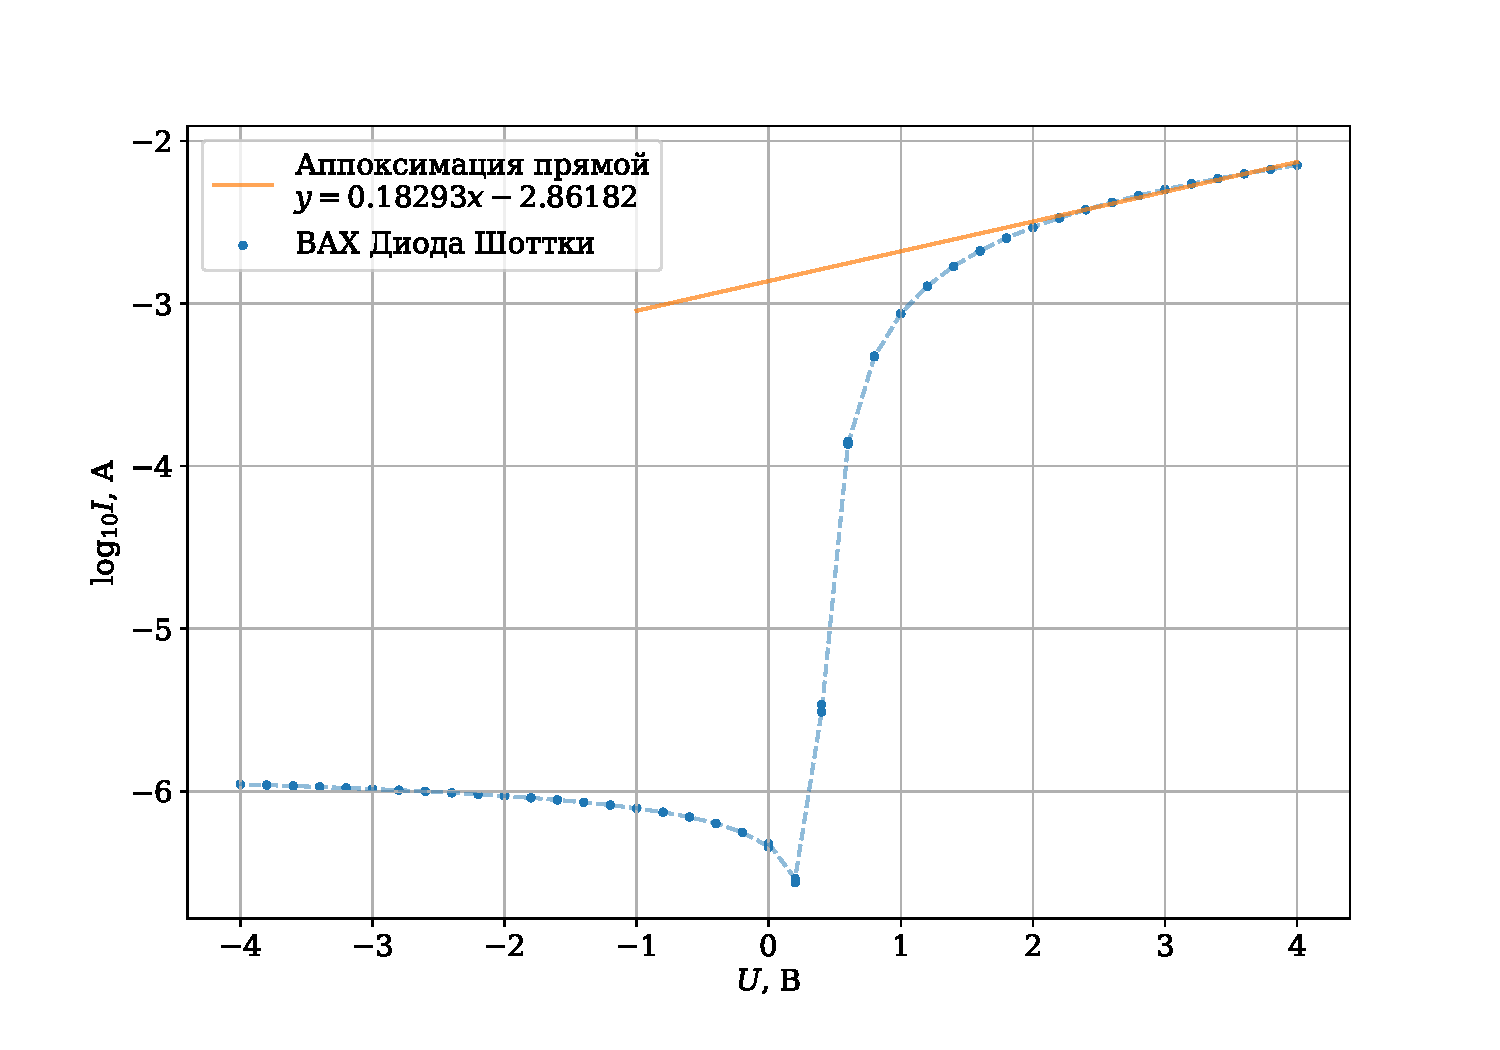
\includegraphics[width=\textwidth]{vac_log10_diode.pdf}
		\caption{ВАХ Шоттки в десятичном логарифмическом масштабе}
		\label{graph2}
	\end{figure}

	\begin{figure}[h!]
		\centering
		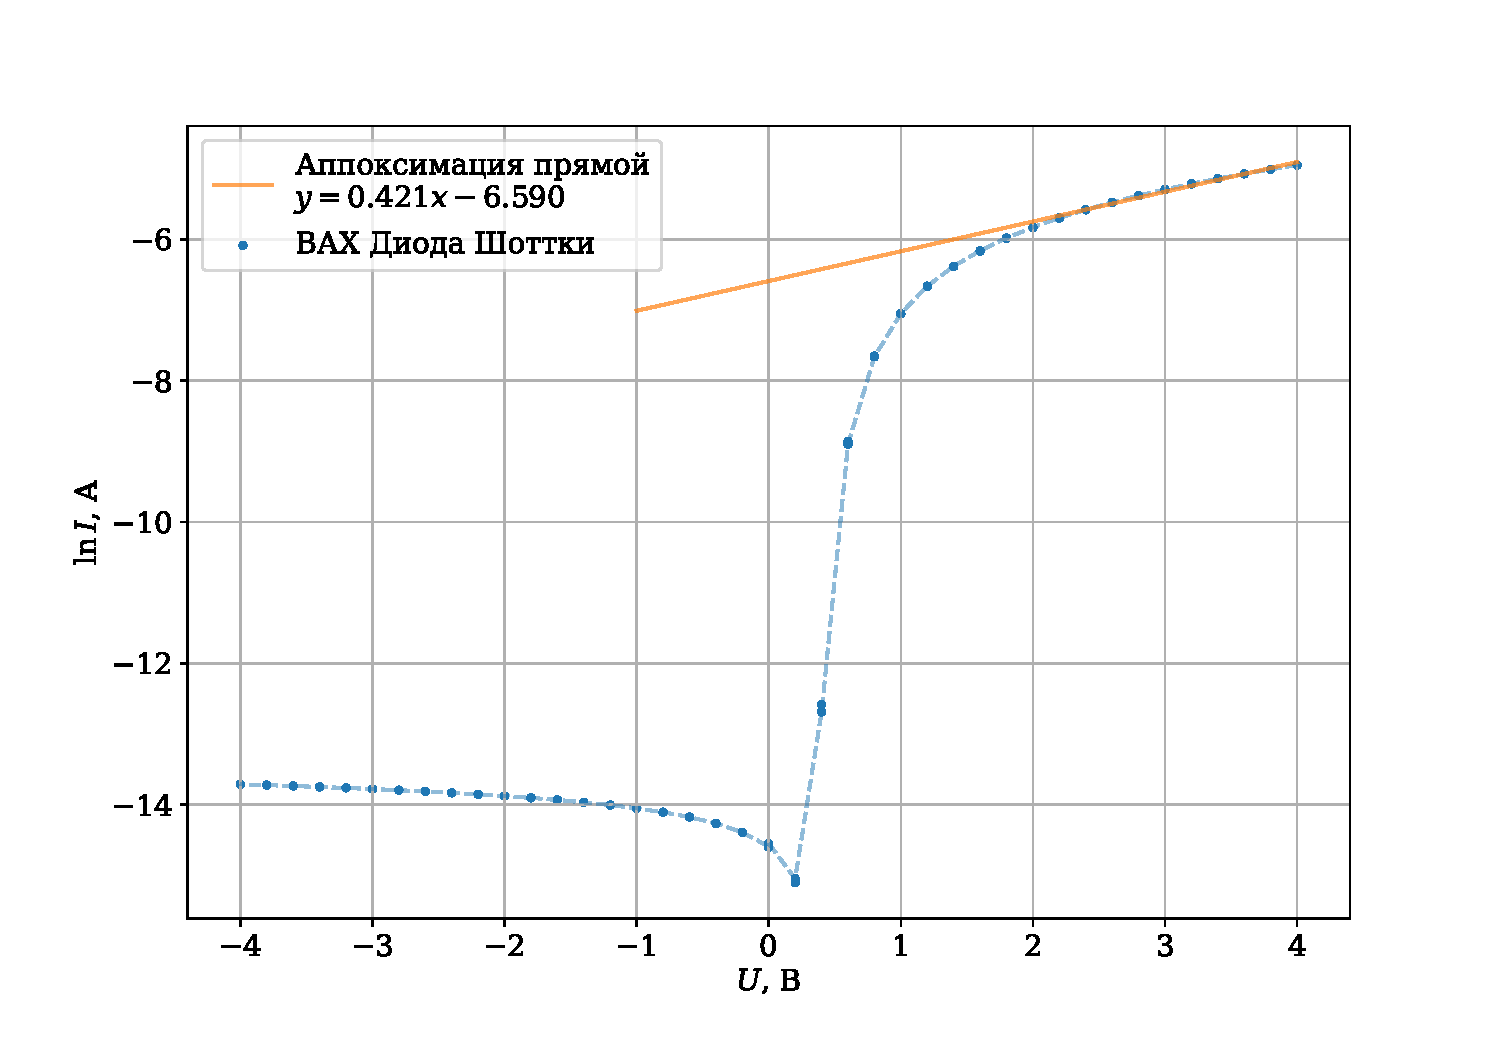
\includegraphics[width=\textwidth]{vac_ln_diode.pdf}
		\caption{ВАХ диода Шоттки в натуральном логарифмическом масштабе}
		\label{graph2}
	\end{figure}


Линейно экстраполируя характеристику к нулевому напряжению, находим $I_0 $:
\[I_0= -6.59 \pm 0,05\]
Получили $I_0$ с точностью до знака. Минус означает, что ток течёт в противоположном 
направлении с полярностью подключения вольтметра.
Вычислим высоту барьера по формуле:
\begin{equation}
    \varphi_b = k_B T \ln{\frac{SA_0 T^2}{|I_0|}},
\end{equation}
где $S=10^4$ мкм$^2$, $T = 300$ К, $A_0 = 1.20 \cdot 10^{-6} А \cdot м^{-2} \cdot K^{-2}$
Получим:
\[\varphi_b = 0.58 \pm 0.02 \textup{ эВ}\]

\section{Вывод}
В данной работе для выданного нам образца был построен прямолинейный участок ВАХ выпрямляющего контакта в полулогарифмическом масштабе и вычислена величина высоты энергетического барьера $\varphi_b = 0.58 \pm 0.02 \textup{ эВ}$.\\


\begin{figure}
\centering
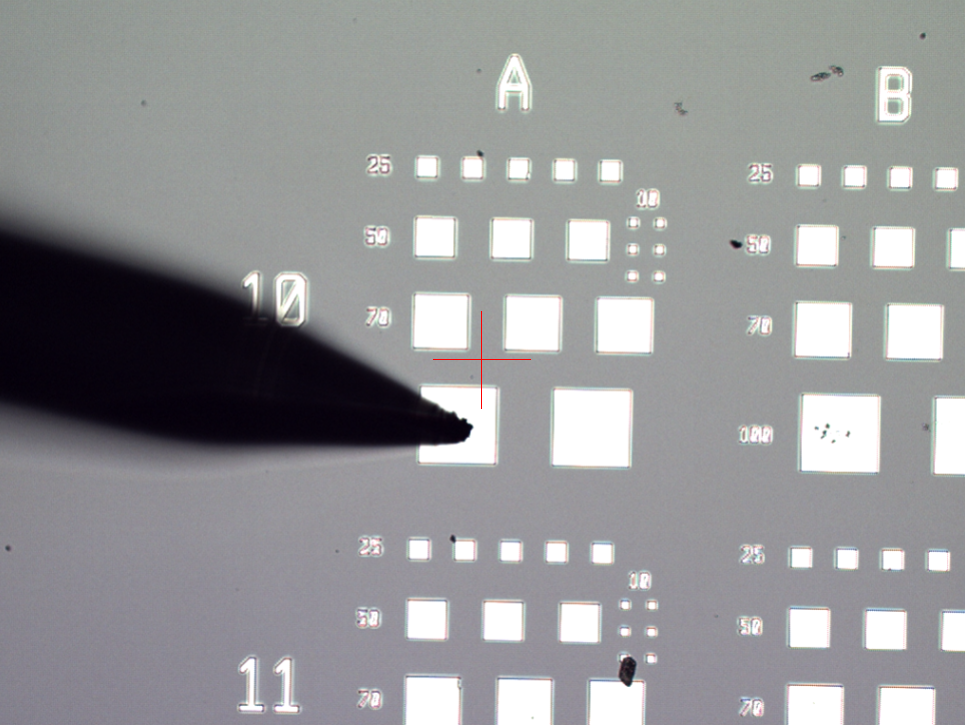
\includegraphics[width=0.5\textwidth]{microscope.png}
\caption{Диод Шоттки под микроскопом}
\label{fig:micro}
\end{figure}




\medskip\hrule\medskip


\end{document}
